\documentclass[tikz,border=4pt]{standalone}
\usepackage{amsmath,amssymb}
\usetikzlibrary{positioning,arrows.meta,fit,backgrounds}
\begin{document}
\sffamily\small
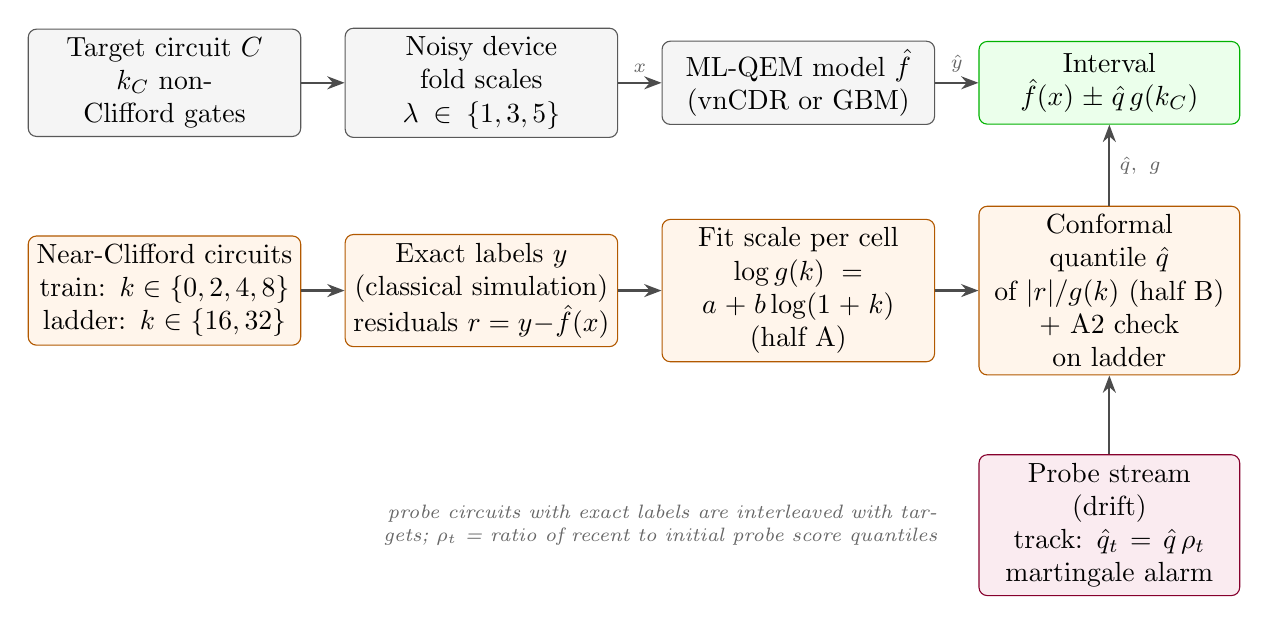
\begin{tikzpicture}[
  box/.style={draw=#1!70!black, fill=#1!8, rounded corners=3pt, align=center, minimum height=1.05cm, text width=3.25cm, inner sep=3pt},
  box/.default=blue,
  arr/.style={-{Stealth[length=2.2mm]}, thick, draw=black!70},
  lab/.style={font=\scriptsize\itshape, text=black!60}]
% top row: deployment of the ML-QEM model
\node[box=gray] (tgt) {Target circuit $C$\\ $k_C$ non-Clifford gates};
\node[box=gray, right=0.55cm of tgt] (dev) {Noisy device\\ fold scales $\lambda\in\{1,3,5\}$};
\node[box=gray, right=0.55cm of dev] (mod) {ML-QEM model $\hat f$\\ (vnCDR or GBM)};
\node[box=green, right=0.55cm of mod, text width=3.1cm] (out) {Interval\\ $\hat f(x)\pm \hat q\, g(k_C)$};
\draw[arr] (tgt) -- (dev);
\draw[arr] (dev) -- node[above, lab]{$x$} (mod);
\draw[arr] (mod) -- node[above, lab]{$\hat y$} (out);
% bottom row: calibration with the k-ladder
\node[box=orange, below=1.25cm of tgt] (nc) {Near-Clifford circuits\\ train: $k\in\{0,2,4,8\}$\\ ladder: $k\in\{16,32\}$};
\node[box=orange, right=0.55cm of nc] (lab) {Exact labels $y$\\ (classical simulation)\\ residuals $r=y-\hat f(x)$};
\node[box=orange, right=0.55cm of lab] (g) {Fit scale per cell\\ $\log g(k)=a+b\log(1+k)$\\ (half A)};
\node[box=orange, right=0.55cm of g, text width=3.1cm] (q) {Conformal quantile $\hat q$\\ of $|r|/g(k)$ (half B)\\ + A2 check on ladder};
\draw[arr] (nc) -- (lab);
\draw[arr] (lab) -- (g);
\draw[arr] (g) -- (q);
\draw[arr] (q) -- node[right, lab]{$\hat q,\ g$} (out);
% online layer
\node[box=purple, below=1.0cm of q, text width=3.1cm] (trk) {Probe stream (drift)\\ track: $\hat q_t=\hat q\,\rho_t$\\ martingale alarm};
\draw[arr] (trk) -- (q);
\node[lab, left=0.4cm of trk, text width=7.2cm, align=right] {probe circuits with exact labels are interleaved with targets; $\rho_t$ = ratio of recent to initial probe score quantiles};
\end{tikzpicture}
\end{document}
